\chapter{Implementation}
This chapter describes some parts of the software implementation.
For further details, see the documentation.

\section{Algorithms}
As mentioned in the introduction, section \ref{sec:externalCollaboration}, the consultants deliver the data algorithms to analyse the measurements from the racket.
These algorithms are written in Python and because of this not directly available to the \glsi{node} environment on the back-end and JavaScript run-time on the front-end.

On the back-end it is possible to execute Python scripts with \glsi{node} if the Python compiler is installed on the server.
It is, however, not possible on the native devices.
Because of this, the algorithms are ported to \gls{typescript} to make them available on both the back-end and front-end.

The algorithms are not optimized or re-factored, but the performance is still increased considerably when running on \glsi{node} as compared to running the scripts in Python.
Early measurements indicate a 10 times performance increase.

\chapter{Security}
This chapter describes the considerations and decisions taken to secure the back-end application.

\section{Authentication}
To make sure that malicious users can not abuse the back-end application, the decision to secure it through authentication was made. 
There was two options for how this could be handled. 

\subsection{The common approach}
This approach is to add a token of sorts to the header of the \gls{http} request. 
The downside of this option when working with \glsi{graphql} is that you can not add a \gls{http} header to your request in \glsi{graphiql} when you query from the browser, unless a browser extension for that specific thing is used. 
It would also not be very transparent or obvious when browsing \glsi{graphiql} that an authentication token is required for certain resources.

\subsection{The Facebook approach}
Facebook uses a root type called a \verb+viewer+ \citep{facebook:viewer}. 
The \verb+viewer+ represent the user making the requests. 
This can be used for several things. 
What we did was add a parameter on the root type \verb+viewer+ so that the \verb+viewer+ takes a token. 
This approach makes it very obvious that the \verb+viewer+ 'area' is restricted and requires a authentication token to access. 
Every resource that requires an authenticated user will then be underneath the \verb+viewer+ type and every other endpoint are exposed outside the \verb+viewer+ object. 
On figure \ref{fig:queryViewer} this is illustrated.

\graphic{0.6}{query}{API documentation for the root query with the viewer and login queries returning the viewer type}{fig:queryViewer}

Notice that both of them returns a \verb+viewer+ type. 
When logging in, the same \verb+viewer+ as you can get when asking for the \verb+viewer+ with your token, is returned. 
This is to save a round-trip after logging on, figure \ref{fig:loginSequence2}. 
Another approach is to \verb+login+ and only receive a token which can then be use to query for the \verb+viewer+. 
But that approach is slower since it requires two round-trips as shown on figure \ref{fig:loginSequence1}.

\begin{figure}
    \centering
    \begin{subfigure}[b]{0.45\textwidth}
        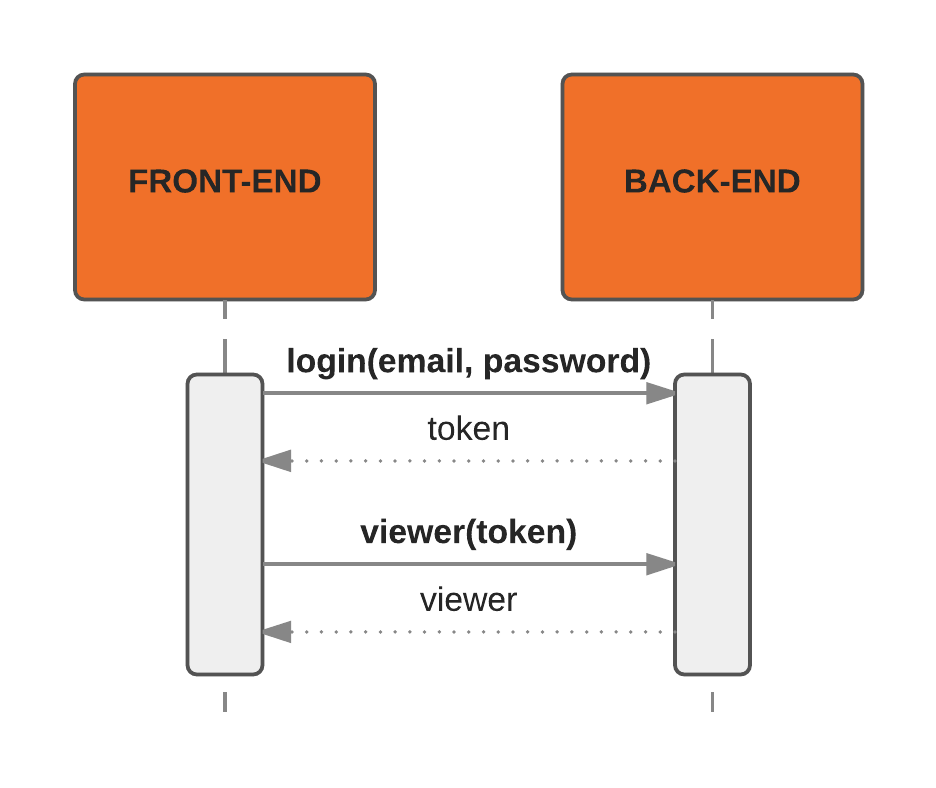
\includegraphics[width=\textwidth]{graphics/loginSequence1}
        \caption{Login returns token to further query with}
        \label{fig:loginSequence1}
    \end{subfigure}
    \hfill
    \begin{subfigure}[b]{0.45\textwidth}
        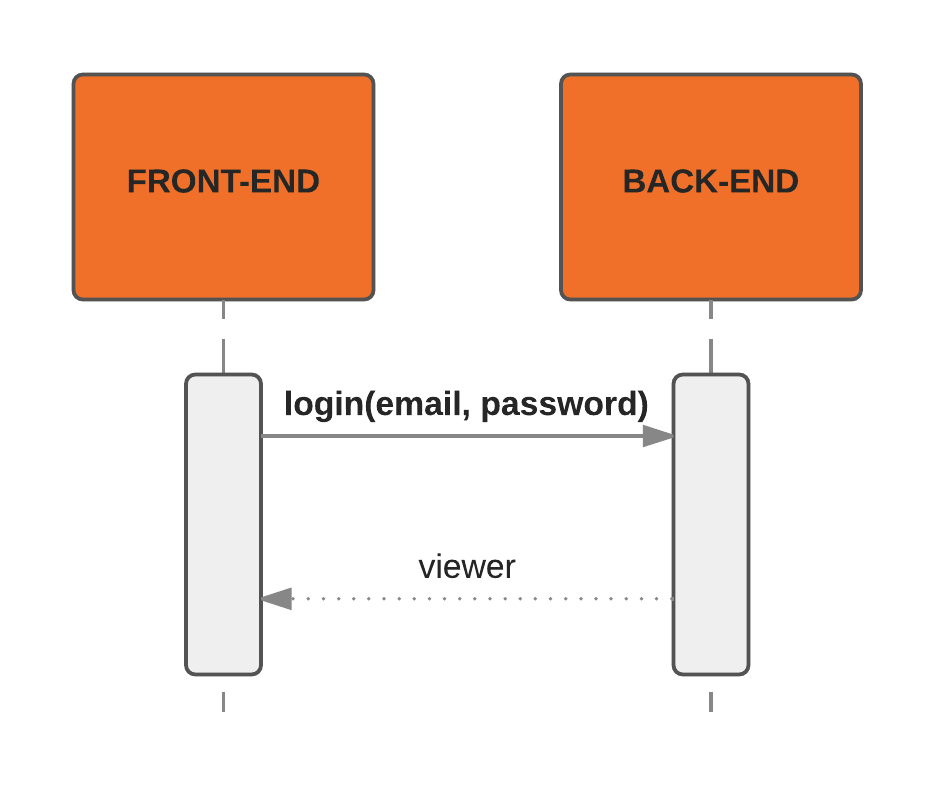
\includegraphics[width=\textwidth]{graphics/loginSequence2}
        \caption{Login returns viewer for direct access}
        \label{fig:loginSequence2}
    \end{subfigure}
    \caption{Authentication token request flows}
\end{figure}

The most important queries to get behind authentication is the mutations since they are the queries that manipulate data. 
So all the mutations are hidden behind a \verb+MutationViewer+. 
This is shown on figure \ref{fig:mutationViewer}. 
When passing the token to the viewer, it is checked in the database and the user owning the token, if any, is then passed down the graph so that the queries below the viewer know exactly who the user is. 

\graphic{0.6}{mutation}{API documentation for the MutationViewer type}{fig:mutationViewer}

\subsection{Token generation}
The token is generated on login and removed on logout. 
An \verb+npm+ package named \verb+node-uuid+ is used to generate an RFC4122 v4 UUID, which is then stored with the user. 

The odds of creating duplicate tokens when using RFC4122 v4 is extremely small. 
On average it would take a few trillions of UUIDs to generate two duplicate tokens \citep{authentication:uuid}.


\chapter{Dependencies}
\label{ch:dependencies}
The project utilizes several external dependencies on both the front- and back-end applications.
They are managed with the package manager \glsi{npm} for \glsi{node}.

All but one of these dependencies are free to use and licensed with \gls{oss} licenses, that grant the user rights to use and in most cases modify and copy the source code.
They are all listed in the documentation, chapter \ref{doc:ch:dependencies}.

One dependency is a commercial product and not free to use, namely the \verb+nativescript-telerik-ui-pro+ package.
The costs of the package is kr. 1400 (\$199) \citep{dependencies:nativescript} per developer, but is provided by Telerik free of charge for this project on a student license.

The project utilizes only a subset of this package and may be too costly for the final product.
To avoid this cost, an effort could be made into finding an alternative product that can provide the same functionality, but without the commercial license.

